\documentclass{beamer}
\usepackage[version=4]{mhchem} 
\usepackage{tikz}


\usetheme{Madrid}
\usecolortheme{beaver}

\title{Unit 3}
\subtitle{Modeling Atomic Structure}
\author{Mr. Maxwell}
\institute{PACS}
\date{\today}


\begin{document}

\frame{\titlepage}

\frame{\tableofcontents}

\section{Atomic Structure}

\subsection{Atomic Number}

\begin{frame}
    \frametitle{Atomic Number}
\onslide The 
 \pause \alert{atomic number}
 \onslide is the number of 
 \pause \alert{protons} 
 \onslide in the nucleus of an atom.
\end{frame}

\subsection{Mass Number}
\begin{frame}
    \frametitle{Atomic Mass}
    \onslide The 
     \pause \alert{mass number}
     \onslide the total number of
     \pause \alert{protons} 
     \onslide and
     \pause \alert{neutrons} 
     \onslide in the nucleus of an atom.
    \end{frame}


\subsection{Hydrogen}    
\begin{frame}
    \frametitle{Hydrogen}
    $$\ce{^{\alert{1}}_{}H}$$

    \pause What does the \alert{1} mean?\\

    \pause 1 is the total number of neutrons and protons.

    \vspace{1cm}

    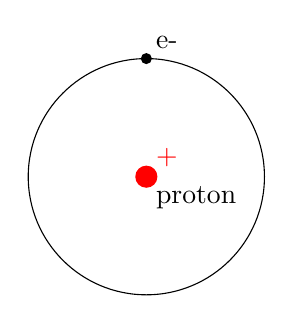
\begin{tikzpicture}
        \coordinate (center) at (0,0);
        \def\radius{1.5cm}
        % a circle
        \draw (center) circle[radius=\radius];
        \fill (center) circle[radius=2pt] node[below right] {proton};
      
        % a random point of the circle
 
        \fill[red] (center) circle[radius=4pt] node[above right] {+};
        \fill[black] (center) ++(90:\radius) circle[radius=2pt]  node[above right] {e-};
    \end{tikzpicture}


\end{frame}


\begin{frame}
    \frametitle{Helium}
 $$\ce{^{4}_{2}He}$$

    \pause What does the \alert{4} mean?\\
    \pause \alert{4} is the total number of neutrons and protons.\\
    \pause What does the \alert{2} mean?\\
    \pause \alert{2} is the number of protons.

    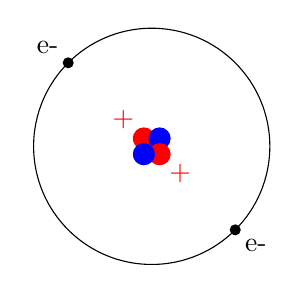
\begin{tikzpicture}

        \coordinate (center) at (0,0);
        \def\radius{1.5cm}
        % a circle
        \draw (center) circle[radius=\radius];

      
        % a random point of the circle
        \fill[red] (-.1, .1) circle[radius=4pt]node[above left] {+};
        \fill[blue] (.1, .1) circle[radius=4pt];
        \fill[red] (.1, -.1) circle[radius=4pt]node[below right] {+};
        \fill[blue] (-.1, -.1) circle[radius=4pt];
        \pause \fill[black] (center) ++(135:\radius) circle[radius=2pt]  node[above left] {e-};
        \pause \fill[black] (center) ++(-45:\radius) circle[radius=2pt] node[below right] {e-};

    \end{tikzpicture}





\end{frame}

\begin{frame}
    \frametitle{Lithium}
 $$\ce{^{7}_{3}Li}$$

    \onslide<1->How many protons does Lithium have? 
    \onslide<2->3 

    \onslide<3-> How many neutrons?\\
    \onslide<4-> $7 - 3 = \onslide<5-> 4 $


    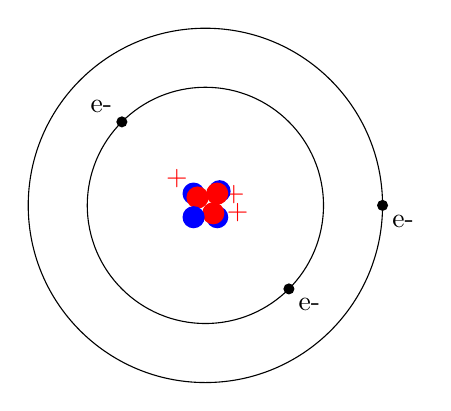
\begin{tikzpicture}

        \coordinate (center) at (0,0);
        \def\radius{1.5cm}
   
        
        \onslide<4->\fill[blue] (-.15, .15) circle[radius=4pt]; 
        \onslide<2->\fill[red] (-.1, .1) circle[radius=4pt]node[above left] {+};  
        \onslide<4->\fill[blue] (.15, -.15) circle[radius=4pt]; 
        \onslide<2->\fill[red] (.1, -.1) circle[radius=4pt]node[above right] {+}; 
        \onslide<4->\fill[blue] (.18, .18) circle[radius=4pt]; 
        \onslide<2->\fill[red] (.15, .15) circle[radius=4pt]node[below right] {+}; 
        \onslide<4->\fill[blue] (-.15, -.15) circle[radius=4pt]; 
        
        
        
        \onslide<6->\draw (center) circle[radius=\radius];
        \onslide<7-> \fill[black] (center) ++(135:\radius) circle[radius=2pt]  node[above left] {e-};
        \onslide<8-> \fill[black] (center) ++(-45:\radius) circle[radius=2pt] node[below right] {e-};
        \onslide<9->\draw (center) circle[radius=\radius*1.5];
        \onslide<10->\fill[black] (center) ++(0:\radius*1.5) circle[radius=2pt] node[below right] {e-};
        
    \end{tikzpicture}

\end{frame}

\subsection{Bohr Model}

\begin{frame}
    \begin{columns}
        \frametitle{Niels Bohr}
        \begin{column}{0.5\textwidth}
            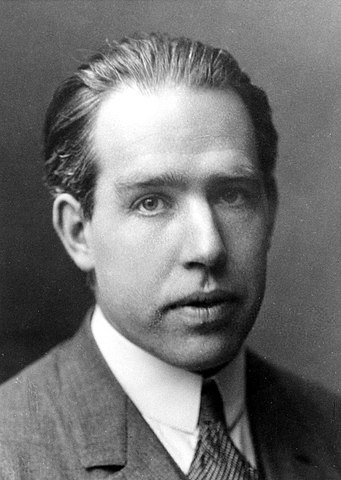
\includegraphics[width=3cm]{../../../../public/images/chemists/Bohr.jpg}
        \end{column}
        \begin{column}{0.5\textwidth}
            The Bohr Model - Bohr proposed that an atom was a nucleus with electrons "orbiting" in different 
            \pause \alert{energy levels}.
            \vspace{1cm}

        
        \end{column}
    \end{columns}
\end{frame}

\subsection{Energy Levels}

\begin{frame}
    \frametitle{Energy Levels}
    \onslide Electrons can only have certain energy values known as
    \pause \alert{energy levels} 
\end{frame}

\begin{frame}
    \frametitle{Energy Levels}
    \onslide The electrons closest to the nucleus have the 
    \pause \alert{lowest} 
    \onslide energy, while those further from away have 
    \pause\alert{higher} 
    \onslide energy.
    \vspace{.5cm}

    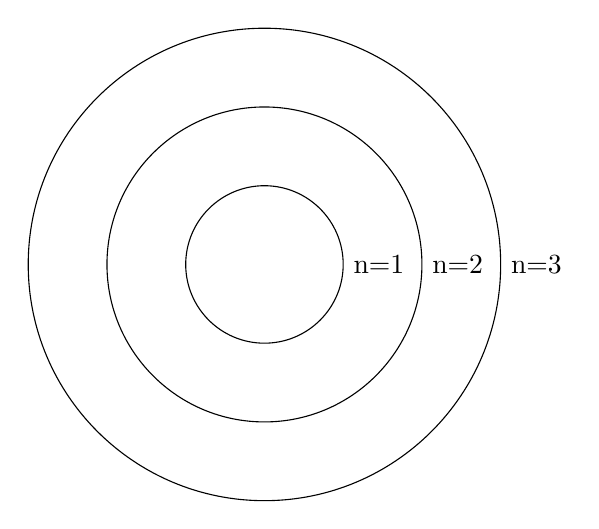
\begin{tikzpicture}
    \foreach \r/\c in {1/n=1, 2/n=2, 3/n=3} 
    {
      \pause \node[circle, draw, minimum size=2*\r cm,label=right:\c] {};
    }
      \end{tikzpicture}
    
\end{frame}

\subsection{The Periodic Table}

\begin{frame}
    \frametitle{Energy Levels and the Periodic Table}
    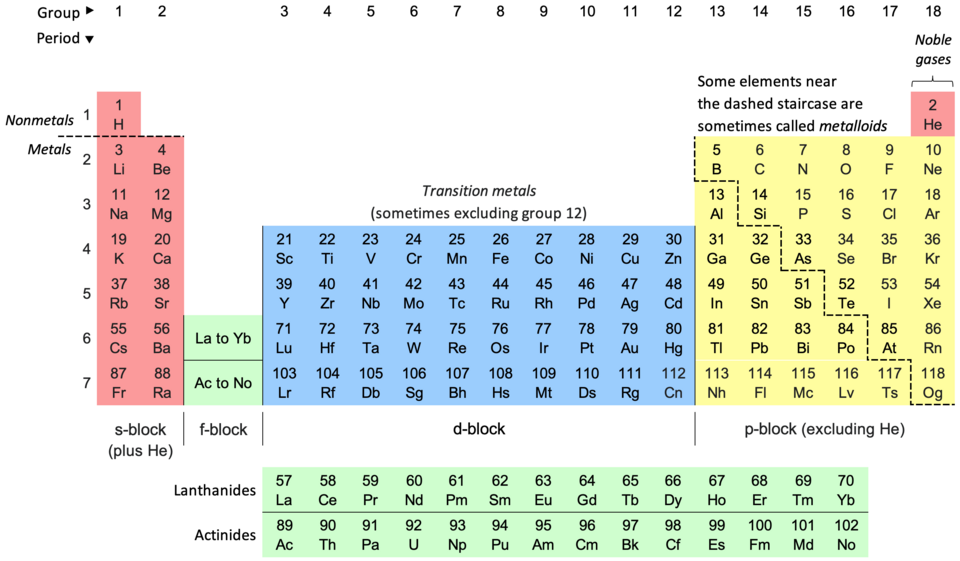
\includegraphics[width=10cm]{../../../../public/images/pTable.png}
\end{frame}

\begin{frame}
    \frametitle{Energy Level of Hydrogen}
    \begin{columns}
        
        \begin{column}{0.5\textwidth}
            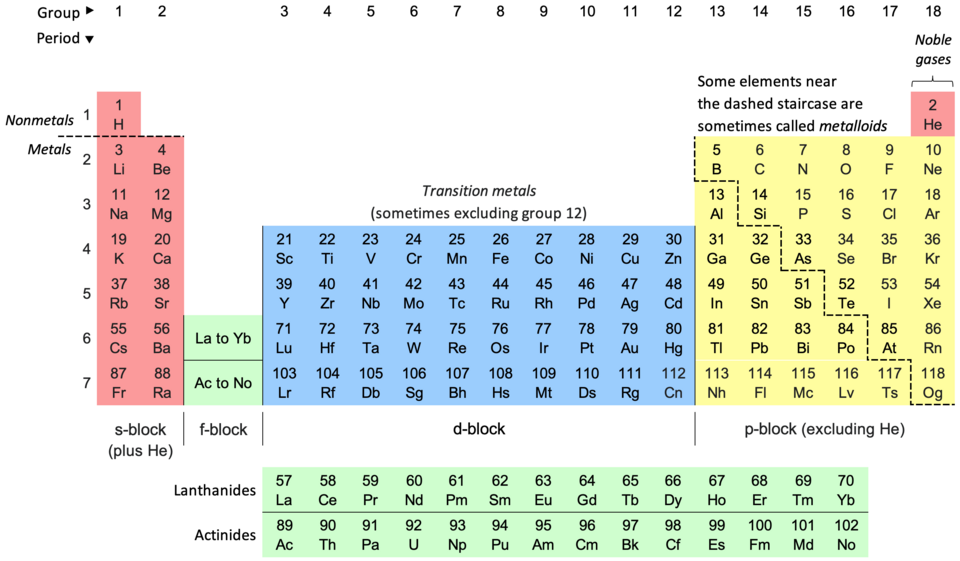
\includegraphics[width=6cm]{../../../../public/images/pTable.png}
            
        \end{column}
        \begin{column}{0.5\textwidth}

            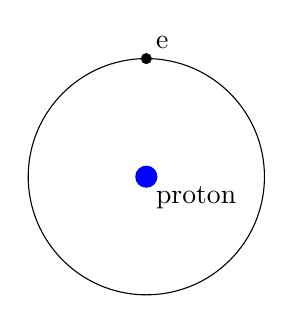
\begin{tikzpicture}
                \coordinate (center) at (0,0);
                \def\radius{1.5cm}
                % a circle
                \draw (center) circle[radius=\radius];
                \fill (center) circle[radius=2pt] node[below right] {proton};
              
                % a random point of the circle
         
                \fill[blue] (center) circle[radius=4pt];
                \fill[black] (center) ++(90:\radius) circle[radius=2pt]  node[above right] {e};
            \end{tikzpicture}
            
        \end{column}
    \end{columns}

\end{frame}

\begin{frame}
    \frametitle{Energy Level of Lithium}
    \begin{columns}
        
        \begin{column}{0.5\textwidth}
            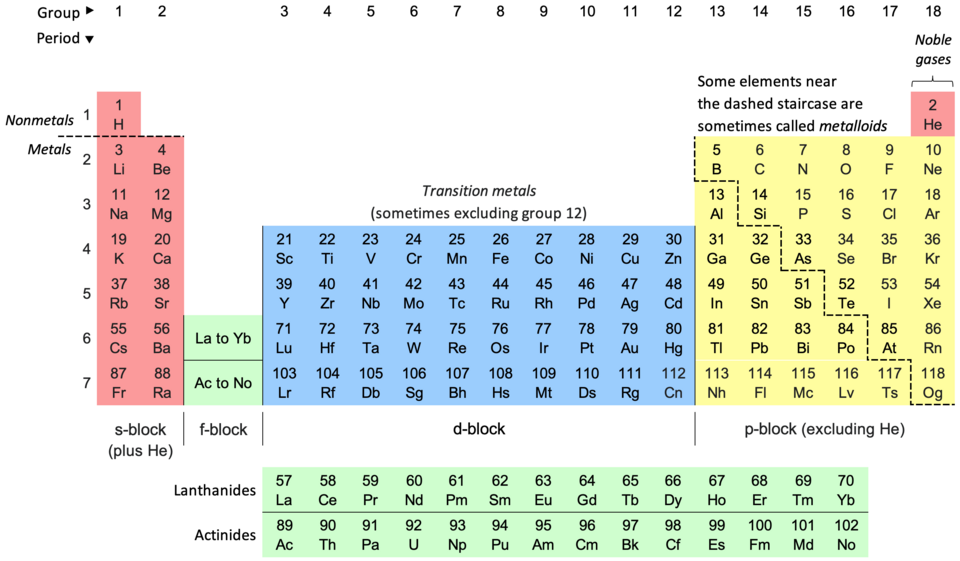
\includegraphics[width=6cm]{../../../../public/images/pTable.png}
            
        \end{column}
        \begin{column}{0.5\textwidth}
            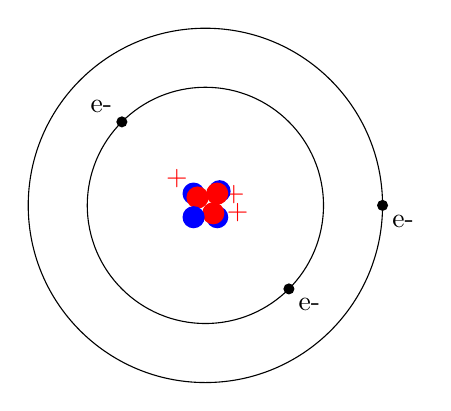
\begin{tikzpicture}
                \coordinate (center) at (0,0);
                \def\radius{1.5cm}
           
                
                \onslide<4->\fill[blue] (-.15, .15) circle[radius=4pt]; 
                \onslide<2->\fill[red] (-.1, .1) circle[radius=4pt]node[above left] {+};  
                \onslide<4->\fill[blue] (.15, -.15) circle[radius=4pt]; 
                \onslide<2->\fill[red] (.1, -.1) circle[radius=4pt]node[above right] {+}; 
                \onslide<4->\fill[blue] (.18, .18) circle[radius=4pt]; 
                \onslide<2->\fill[red] (.15, .15) circle[radius=4pt]node[below right] {+}; 
                \onslide<4->\fill[blue] (-.15, -.15) circle[radius=4pt]; 
                
                
                
                \onslide<6->\draw (center) circle[radius=\radius];
                \onslide<7-> \fill[black] (center) ++(135:\radius) circle[radius=2pt]  node[above left] {e-};
                \onslide<8-> \fill[black] (center) ++(-45:\radius) circle[radius=2pt] node[below right] {e-};
                \onslide<9->\draw (center) circle[radius=\radius*1.5];
                \onslide<10->\fill[black] (center) ++(0:\radius*1.5) circle[radius=2pt] node[below right] {e-};
                
            \end{tikzpicture}
            
        \end{column}
    \end{columns}

\end{frame}

\begin{frame}
    \frametitle{Energy Level of Sodium}
    \begin{columns}
        
        \begin{column}{0.5\textwidth}
            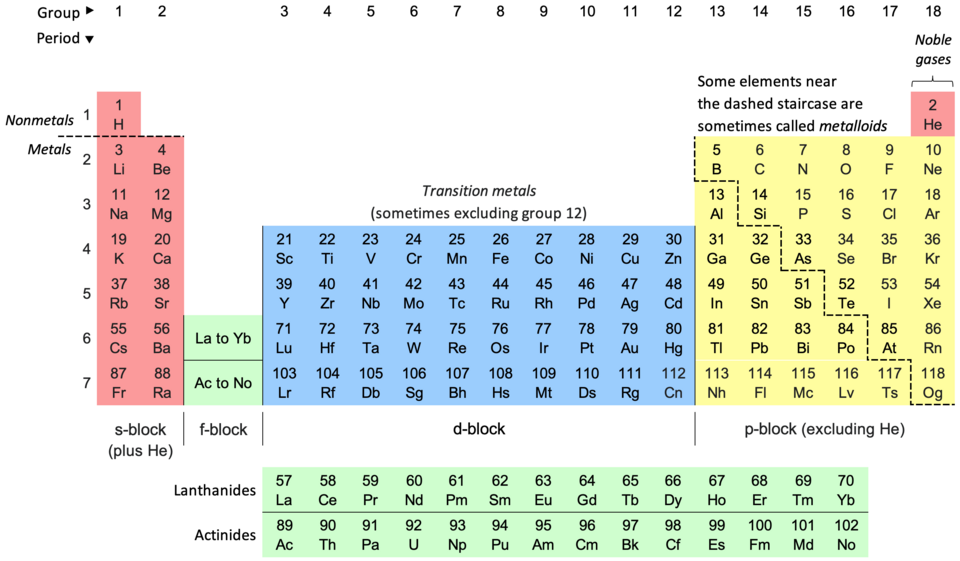
\includegraphics[width=6cm]{../../../../public/images/pTable.png}
            
        \end{column}
        \begin{column}{0.5\textwidth}
            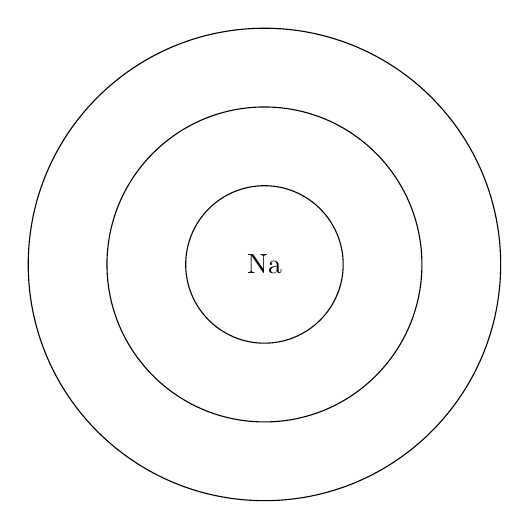
\begin{tikzpicture}
                \foreach \r/\c in {1/Na, 2/, 3/} { \pause \node[circle, draw, minimum size=2*\r cm,label=center:\c] {};}
                \end{tikzpicture}
            
        \end{column}
    \end{columns}

\end{frame}

\subsection{Valence Electrons}



\end{document}